\documentclass[9pt,letterpaper,onecolumn]{rho-class/rho}
\usepackage[spanish,es-nodecimaldot,es-noindentfirst]{babel}
\usepackage{graphicx}
\usepackage{float}
\setlength{\parindent}{0pt}  % Elimina la sangría
\usepackage[utf8]{inputenc}
\usepackage[T1]{fontenc}
\setbool{rho-abstract}{true} % Set false to hide the abstract
\setbool{corres-info}{true} % Set false to hide the corresponding author section
\addbibresource{rho.bib}

%----------------------------------------------------------
% TITLE
%----------------------------------------------------------

%\journalname{Example Template}
\title{Fly: Motor de búsqueda}

%----------------------------------------------------------
% AUTHORS AND AFFILIATIONS
%----------------------------------------------------------
\author[$\dagger$]{Franco Aguilar}
\author[$\dagger$]{Milton Hernandez}
\author[$\dagger$]{Iván Mansilla}
\author[$\dagger$]{Ayrton Morrison}


%----------------------------------------------------------

%\affil[1]{Affiliation of author one}
%\affil[2]{Affiliation of author two}
%\affil[3]{Affiliation of author three}
\affil[$\dagger$]{Universidad de Magallanes}

%----------------------------------------------------------
% DATES
%----------------------------------------------------------

\dates{Este informe fue compilado el \today}

%----------------------------------------------------------
% FOOTER INFORMATION
%----------------------------------------------------------

%\leadauthor{Author last name et al.}
%\footinfo{Creative Commons CC BY 4.0}
\smalltitle{Estructuras de datos}
%\institution{College name}
\theday{\today} %\today

%----------------------------------------------------------
% ARTICLE INFORMATION
%----------------------------------------------------------

%\corres{Provide the corresponding author information and publisher here.}
%\email{example@organization.com.}
%\doi{\url{https://www.doi.org/exampledoi/XXXXXXXXXX}}

%\received{March 20, 2024}
%\revised{April 16, 2024}
%\accepted{April 20, 2024}
%\published{May 21, 2024}

%\license{Rho LaTeX Class \ccLogo\ This document is licensed under Creative Commons CC BY 4.0.}

%----------------------------------------------------------
% ABSTRACT
%----------------------------------------------------------

\begin{abstract}
    Fly es un sistema de recuperación de información que indexa documentos de texto plano enlazados entre sí. Para esto usa diferentes estructuras de datos que facilitan una rápida recopilación de información, la búsqueda y la navegación entre los archivos. En el presente informe encontrará una descripción detallada de la implementación de Fly.
\end{abstract}

%----------------------------------------------------------

\keywords{Índice invertido, Listas enlazadas simples, PageRank, Tablas hash}

%----------------------------------------------------------
\begin{document}
    \maketitle
    \thispagestyle{firststyle}
    \tableofcontents
    %\linenumbers
    %----------------------------------------------------------


    \newpage
    \section{Introducción}
Un motor de búsqueda es una herramienta que permite buscar y recuperar datos en una colección de archivos.

Particularmente, \textit{Fly} es un motor de búsqueda que indexa documentos enlazados entre sí mediante \textit{WikiLinks}\footnote{Un WikiLink es un tipo de enlace entre documentos de texto usado en la aplicación \href{https://obsidian.md/}{Obsidian.md} consistente en el siguiente formato: \texttt{[[nombre del archivo enlazado|Alias para el archivo de ser necesario]]}. Este formato tiene diversas facilidades para un sistema de archivos con las características deseadas razón por la cuál fue utilizado en este proyecto.}. De estos archivos este motor extrae todas las palabras \textit{relevantes} permitiendo al usuario buscar una palabra y encontrar las coincidencias de la misma a lo largo del sistema de archivos. Para llevar a cabo esta tarea, Fly utiliza técnicas como el \textit{índice invertido} (para la indexación de palabras) y el \textit{PageRank} (para la jerarquización de los archivos analizados).

Las principales funciones de \textit{Fly} son:
\begin{enumerate}
    \item Generar un grafo con los archivos de un directorio, almacenando en cada nodo un archivo y relacionándolo con los archivos que lo enlazan y aquellos a los que se enlaza.
    \item Generar un índice invertido para almacenar la información de cada palabra relevante en el sistema de archivos.
    \item Calcular el nivel de importancia de cada uno de los archivos en el grafo, utilizando el algoritmo de PageRank.
    \item Realizar búsquedas eficientes sobre el índice invertido y el grafo permitiendo al usuario encontrar coincidencias entre palabras y sus ubicaciones en cada archivo donde aparecen.
\end{enumerate}

Todas estas funciones se implementaron mediante el uso de estructuras de datos tales como grafos, listas enlazadas y tablas hash.

El presente informe describe el proceso de desarrollo e implementación de Fly, detallando las decisiones de diseño y las técnicas utilizadas para crear un sistema eficiente de busqueda y recuperación de información.
    \section{Objetivos}
\rhostart{}

En este proyecto, se tiene el objetivo de crear un programa eficiente y rápido en la búsqueda y recuperación de información, utilizando estructuras de datos como grafos, listas enlazadas y tablas hash, y además aplicar técnicas de investigación para implementar un sistema de búsqueda eficiente.

\subsection{Objetivos secundarios}
\begin{enumerate}
\item \textbf{Utilización de estructura de datos:} Crear estructuras de datos eficientes para almacenar y procesar información mediante el uso de listas enlazadas, tablas hash, grafos y manejo de archivos.
\item \textbf{Optimización de código:} Optimizar el código para mejorar su eficiencia y rendimiento.
\item \textbf{Trabajo en equipo:} Reforzar el trabajo en equipo y la comunicación entre los miembros del equipo para asignar tareas y resolver conflictos.
\item \textbf{Eficiencia:} Conseguir tiempos cortos de ejecución mediante algoritmos de búsqueda eficientes.
\end{enumerate}
    \newpage
    \section{Planteamiento del desarrollo del proyecto}
\rhostart{}
    \newpage
    \section{Implementación}
\rhostart{}

La implementación del programa se realizó mediante el lenguaje de programación C. Las funciones necesarias fueron implementadas en archivos separados según su funcionalidad. El código fue compilado a través de un \texttt{Makefile}, el cual se encuentra en el directorio raíz.

\subsection{Estructura de directorios}
Dentro del directorio \texttt{src} se encuentran los siguientes archivos:

\begin{itemize}
    \item \texttt{errors.c}: Contiene las funciones de gestión de errores.
    \item \texttt{files.c}: Contiene las funciones de gestión de archivos.
    \item \texttt{graph.c}: Contiene las funciones de gestión de grafos.
    \item \texttt{hash.c}: Contiene las funciones de gestión de tablas hash.
    \item \texttt{link\_list.c:} Contiene las funciones de gestión de listas enlazadas.
    \item \texttt{main.c}: Contiene el código principal del programa.
    \item \texttt{page\_rank.c}: Contiene las funciones de calculación de PageRank.
    \item \texttt{reverse\_index.c}: Contiene las funciones de gestión del índice invertido.
    \item \texttt{stop\_words.c}: Contiene las funciones de gestión de stop words.
    \item \texttt{timer.c}: Contiene las funciones de gestión de tiempo de ejecución.
    \item \texttt{utilities.c}: Contiene las funciones de utilidad del programa.
\end{itemize}

Por otro lado, en la carpeta \texttt{testing} se encuentran archivos para el testeo del programa:
\begin{itemize}
    \item \texttt{spanish.txt}: Contiene una lista de stop words en español.
    \item \texttt{test.txt}: Script de \textit{Python} que recupera de \textit{Wikipedia} artículos aleatorios.
\end{itemize}


\subsection{Estructuras de datos}

\subsubsection{Índice invertido}
Para el índice invertido se optó finalmente por utilizar una \textbf{tabla hash} para almacenar las palabras, permitiendo así una búsqueda de orden $O(1)$. Sin embargo, acá surgieron algunos inconvenientes, como la necesidad de manejar posibles colisiones y el límite de memoria que trae consigo los arreglos. Para solucionar esto, se optó que cada celda de esta tabla hash contenga una \textbf{lista enlazada simple}, en la cual será en donde realmente se almacenarán las palabras asociadas a un hash key. Esto permite una búsqueda más eficiente y sin un límite de memoria.

Por otro lado, para poder relacionar un archivo con una palabra se hizo que cada palabra además almacene consigo otra \textbf{lista enlazada simple}, en la cual se almacenarán los archivos que contienen dicha palabra.

\begin{figure}[h!]
    \centering
    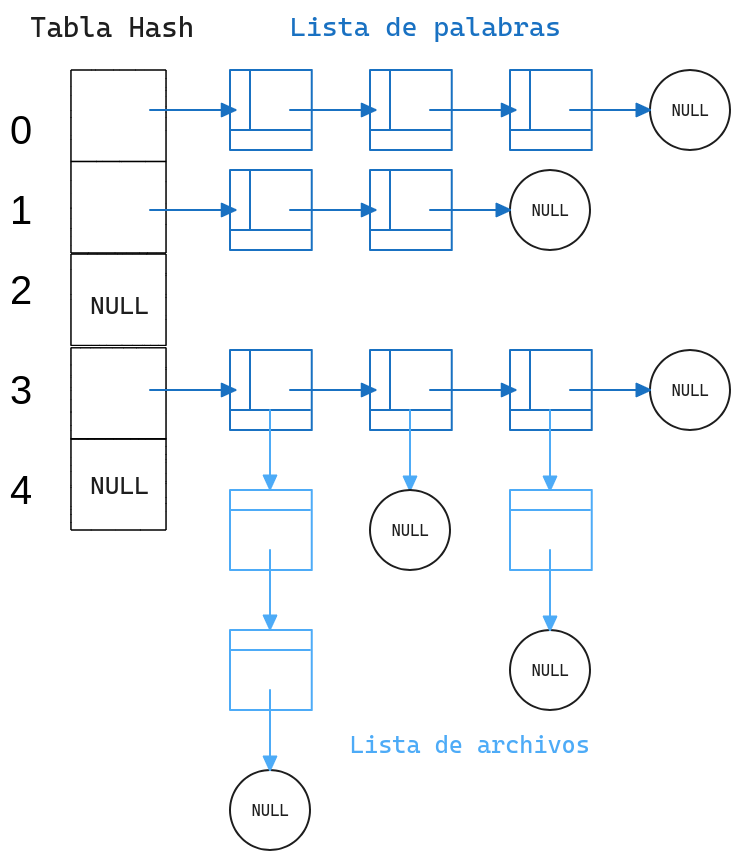
\includegraphics[width=0.3\textwidth]{src/figures/reverse_index.png}
    \caption{Esquema de la estructura de datos del índice invertido}
\end{figure}

\subsubsection{Grafos}

\subsection{PageRank}

\subsection{Manejo de archivos}
Para el manejo de archivos se optó por utilizar una \textbf{lista enlazada simple} para almacenar los archivos, en la cual cada archivo se almacena en una celda de la lista. Esto permite una búsqueda más eficiente y sin un límite de memoria. Además, para poder identificar y procesar los archivos del directorio y sus sub-directorios se utilizó la librería \textbf{dirent.h}.

La librería \textbf{dirent.h} es una librería de C que permite leer los archivos de un directorio, y que proporciona una estructura llamada \textbf{struct dirent} que contiene información sobre cada archivo, como por ejemplo su nombre (con extensión), su tipo (archivo o directorio) y su identificador (ID).

En el caso de existir un sub-directorio dentro del directorio de entrada, se procesará recursivamente, añadiendo cada archivo que se encuentre en dicho directorio a la lista de archivos.

Por último para poder identificar los archivos que contienen texto plano, se utilizó una función para extraer el nombre sin extensión y a su vez verificar si el archivo es de texto plano a traves de su extensión.

\subsection{implementaciones extras}
Se implementó un temporizador para medir los tiempos de ejecución de las funciones y así analizar y mejorar el código(solo para testing).

También se utilizó \textbf{mergeSort} para ordenar (de mayor a menor) el PageRank de los archivos, para tener una mejor visualización de los resultados.
    \newpage
    \section{Gestión del equipo de trabajo}
\rhostart{}
    \newpage
    \section{Posibles Mejoras a futuro}
\rhostart{}

    \newpage
    \section{Ejemplo de uso}

Dentro de esta sección se busca explicar parte del cómo sería una manera correcta de utilizar \textit{Fly} para buscar y mostrar coincidencias de una palabra en particular.

\subsection{Preparación de los archivos}
A la hora de utilizar \textit{Fly} se debe tener en cuenta que el programa lee solamente archivos de texto plano; particularmente se recomienda el uso de archivos tipo \texttt{Markdown}(.md) para los que el programa está especialmente diseñado.

Como fue mencionado anteriormente Fly reconoce enlaces mediante el uso de WikiLinks, a continuación se muestran algunos ejemplos de enlaces válidos:
\begin{itemize}
    \item \texttt{[[nombre archivo enlazado]]}
    \item \texttt{[[nombre archivo enlazado.extension]]}
    \item \texttt{[[/ruta/al/archivo/enlazado/nombre archivo enlazado.extension]]}
    \item \texttt{[[nombre archivo enlazado\#sección del archivo]]} (esto es usado en aplicaciones como \href{https://obsidian.md/}{Obsidian.md} para generar un link a una sección del archivo).
    \item \texttt{[[nombre archivo enlazado|Alias para el archivo]]} (esto es usado en aplicaciones como Obsidian para generar un link y que aparezca un texto diferente al nombre del archivo).
\end{itemize}

Por lo general combinaciones de este tipo de links (alias con secciones, rutas, extensiones, etc) son válidas dentro de \textit{Fly}.

\subsection{Uso del programa}
Una vez con los archivos correctamente formateados se puede ejecutar \textit{Fly} desde la carpeta raíz del repositorio del proyecto con el comando \texttt{./build/fly.out -d <directorio a procesar>} lo cuál procesará el directorio indicado y permitirá ingresar palabras para su búsqueda dentro de los archivos procesados.

\subsection{Prueba de estrés del programa}
\textit{Fly} fue probado con un dataset de $856$ archivos construidos sobre Obsidian. Con este dataset se obtuvo un tiempo de procesamiento promedio menor a $1s$ para procesar todos los archivos y permitir la interacción del usuario. Posterior a esto los tiempos de respuesta de Fly son realmente cortos, lo que demuestra la eficiencia del programa.

Adicionalmente se ejecutó el programa bajo la herramienta \texttt{Valgrind} diseñada para encontrar fugas de memoria (herramienta muy útil para la depuración de errores durante el desarrollo de este programa), y se obtuvo un resultado de $0$ fugas de memoria y un total de $\approx 24Mb$ de memoria utilizada durante su ejecución, lo que indica el correcto funcionamiento del programa.
    \newpage
    \section{Conclusiones}
\rhostart{}

    \newpage
    \nocite{*}
    \printbibliography
\end{document}